% Jacob Neumann

% DOCUMENT CLASS AND PACKAGE USE
    \documentclass[aspectratio=169, handout]{beamer}

    % Establish the colorlambda boolean, to control whether the lambda is solid color (true), or the same as the picture (false)
    \newif\ifcolorlambda
    \colorlambdafalse % DEFAULT: false

    % Use auxcolor for syntax highlighting
    \newif\ifuseaux
    \useauxfalse % DEFAULT: false

    % Color settings
    \useauxtrue

    \newcommand{\auxColor}{eb4d4d}     % the color of note boxes and stuff
    \newcommand{\presentColor}{871111} % the primary color of the slide borders
    \newcommand{\bgColor}{c9bbbb}      % the color of the background of the slide
    \newcommand{\darkBg}{8b98ad}
    \newcommand{\lambdaColor}{\auxColor}

    \colorlambdatrue

    \usepackage{comment} % comment blocks
    \usepackage{soul} % strikethrough
    \usepackage{listings} % code
    \usepackage{makecell}
    \usepackage{tcolorbox}
    \usepackage{adjustbox}
    \usepackage{amssymb}% http://ctan.org/pkg/amssymb
    \usepackage{pifont}% http://ctan.org/pkg/pifont
    \usepackage[outline]{contour}
    \usepackage{ stmaryrd }

    \setbeamertemplate{itemize items}[circle]
    % \setbeameroption{show notes on second screen=right}

    \usepackage{lectureSlides}
    %%%%%%%%%%%%%%%%%%%%%%%%%%%%%%%%%%%%%%%%%| <----- Don't make the title any longer than this
    \title{Modules III: Red-Black Trees} % TODO
    \subtitle{Self-balancing in black and crimson} % TODO
    \date{13 July 2023} % TODO
    \author{Brandon Wu} % TODO

    \graphicspath{ {./img/} }
    % DONT FORGET TO PUT [fragile] on frames with codeblocks, specs, etc.
        %\begin{frame}[fragile]
        %\begin{codeblock}
        %fun fact 0 = 1
        %  | fact n = n * fact(n-1)
        %\end{codeblock}
        %\end{frame}

    % INCLUDING codefile:
        % 1. In some file under code/NN (where NN is the lecture id num), include:
    %       (* FRAGMENT KK *)
    %           <CONTENT>
    %       (* END KK *)

    %    Remember to not put anything on the same line as the FRAGMENT or END comment, as that won't be included. KK here is some (not-zero-padded) integer. Note that you MUST have fragments 0,1,...,KK-1 defined in this manner in order for fragment KK to be properly extracted.
        %  2. On the slide where you want code fragment K
                % \smlFrag[color]{KK}
        %     where 'color' is some color string (defaults to 'white'. Don't use presentColor.
    %  3. If you want to offset the line numbers (e.g. have them start at line 5 instead of 1), use
                % \smlFragOffset[color]{KK}{5}

        \def\checkmark{\tikz\fill[green, scale=0.4](0,.35) -- (.25,0) -- (1,.7) -- (.25,.15) -- cycle;}
        \contourlength{.08em}% default is 0.03em
        \newcommand{\cmark}{{\color{green}\ding{51}}}
        \newcommand{\xmark}{{\color{red}\ding{55}}}

        \newcommand{\colr}[1]{{\color{red}#1}}
        \newcommand{\colb}[1]{{\color{black}\textbf{#1}}}

        \newcommand{\goodbox}[2]{
          \begin{tcolorbox}[colframe=green]
            \centering

            \begin{tikzpicture}[#2]
              #1
            \end{tikzpicture}

            \vspace{5pt}

            \textit{Black height invariant: \cmark}

            \vspace{5pt}

            \textit{Red children invariant: \cmark}
          \end{tcolorbox}
        }

        \newcommand{\badbox}[3]{
          \begin{tcolorbox}[colframe=red]
            \centering

            \begin{tikzpicture}
              #1
            \end{tikzpicture}

            \vspace{5pt}

            \textit{Black height invariant: #2}

            \vspace{5pt}

            \textit{Red children invariant: #3}
          \end{tcolorbox}
        }

        \usetikzlibrary{patterns}
        \tikzset{
        level distance=13mm,
        every child/.style={line width=0.3mm},
        black/.style={text=white, circle, draw=black, line width=0.4mm, inner sep=4pt, fill=black!80!white},
        red/.style={text=white, circle, draw=black, line width=0.4mm, inner sep=4pt, fill=red!90!white},
        unknown/.style={text=white, circle, draw=black, line width=0.4mm, inner sep=4pt, preaction={fill, pink!90!black}, pattern=north east lines,distance=0.5pt},
        highlight/.style={draw=yellow!80!white, line width=0.55mm},
        highlight2/.style={draw=magenta, line width=0.45mm},
        highlight3/.style={draw=blue, line width=0.45mm},
        subtree/.style={text=white, circle, draw=black, line width=0.4mm, inner sep=4pt,
          preaction={fill, pink!90!black}, pattern=north east lines, distance=0.5pt, regular polygon, regular polygon sides=3, inner sep = 1pt, font=\small},
        rr/.style={draw=red, line width=0.8mm},
        phighlight2/.style={edge from parent path/.style={highlight2}},
        inline/.style={anchor=base, baseline},
        textnode/.style={circle, draw=black, inner sep=0.05cm}
          }
        % Define a new background color for the boxes
        \definecolor{myboxbg}{HTML}{\bgColor}

        % Customize the tcolorbox settings
        \tcbset{
            colback=myboxbg, % Set the background color for the boxes
            colframe=blue, % Set the color for the frame
            % Add any other desired options here
        }
\begin{document}

% Make it so ./mkWeb works correctly
\ifweb
    \renewcommand{\pause}{}
\fi

\setbeamertemplate{itemize items}[circle]

% SOLID COLOR TITLE (see SETTINGS.sty)
{
\begin{frame}[plain]
    \colorlambdatrue
    \titlepage
\end{frame}
}

\menti{3766 2220}

\begin{frame}[fragile]
  \frametitle{Lesson Plan}

  \tableofcontents
\end{frame}

\begin{frame}[fragile]
  \frametitle{Last time}

  Last time, we iterating several times on implementing \term{generic dictionaries},
  which are dictionaries which can have keys (and data) of arbitrary type.

  \pause
  \vspace{\fill}

  We tried implementing them via passing an explicit comparison function, but found
  that this could lead to unsafety if comparison functions were mixed and matched.

  \pause
  \vspace{\fill}

  We then used \term{functors}, which produce structures from other structures, to
  create a \code{MkDict} functor, which creates a library for dictionaries of a
  particular key type, from a given type and comparison function.
\end{frame}

\sectionSlide{1}{Red-Black Trees}

\begin{frame}[fragile]
  \frametitle{A Signature for Generic Dictionaries}

  Recall the \code{POLY_DICT} signature we used last lecture:

  \begin{codeblock}
    signature POLY_DICT =
      sig
        structure Key : ORD

        (* mapping keys of type Key.t to values of 'a *)
        type 'a t

        val empty : 'a t
        val insert : Key.t * 'a -> 'a t -> 'a t
        val lookup : Key.t -> 'a t -> 'a option
      end
  \end{codeblock}
\end{frame}

\begin{frame}[fragile]
  \frametitle{A Worst-Case Case}

  Recall that our definition of insertion was just via comparing keys to
  root keys, and going left or right depending on the result of that comparison,
  until eventually we found an \code{Empty} node.

  \pause
  \vspace{\fill}

  This is not actually a good way to store data in our dictionaries, because it
  might not be $O(\log n)$ search time! In particular, consider the sequence
  of insertions of inserting ascending numbers, for a tree with nodes of integer
  keys.

  \pause
  \vspace{\fill}

  \begin{center}
  \begin{minipage}{0.15\textwidth}
    \begin{center}
    \begin{tikzpicture}
      [level distance=8mm,
      every node/.style={circle, inner sep=4pt, draw=black!80, thick},
      ]
      \node[draw=none] {(empty)};
    \end{tikzpicture}
    \end{center}
  \end{minipage}
  \pause
  \begin{minipage}{0.09\textwidth}
    \begin{center}
      $\longmapsto$
    \end{center}
  \end{minipage}
  \begin{minipage}{0.15\textwidth}
    \begin{center}
    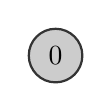
\begin{tikzpicture}
      [level distance=8mm,
      every node/.style={circle, inner sep=4pt, draw=black!80, thick, fill=black!20!white},
      ]
      \node {\code{0}}
        child[missing]
        child[missing];
    \end{tikzpicture}
    \end{center}
  \end{minipage}
  \pause
  \begin{minipage}{0.09\textwidth}
    \begin{center}
      $\longmapsto$
    \end{center}
  \end{minipage}
  \begin{minipage}{0.15\textwidth}
    \begin{center}
    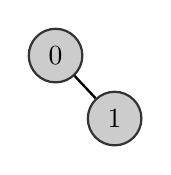
\begin{tikzpicture}
      [level distance=8mm,
      every node/.style={circle, inner sep=4pt, draw=black!80, thick, fill=black!20!white},
      ]
      \node {\code{0}}
        child[missing]
        child{node {\code{1}}
          child[missing]
          child[missing]
      };
    \end{tikzpicture}
    \end{center}
  \end{minipage}
  \pause
  \begin{minipage}{0.09\textwidth}
    \begin{center}
      $\longmapsto$
    \end{center}
  \end{minipage}
  \begin{minipage}{0.15\textwidth}
    \begin{center}
    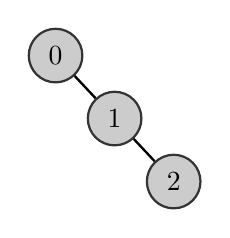
\begin{tikzpicture}
      [level distance=8mm,
      every node/.style={circle, inner sep=4pt, draw=black!80, thick, fill=black!20!white},
      ]
      \node {\code{0}}
        child[missing]
        child{node {\code{1}}
          child[missing]
          child{node {\code{2}}
            child[missing]
            child[missing]
          }
      };
    \end{tikzpicture}
    \end{center}
  \end{minipage}
  \end{center}
\end{frame}

\begin{frame}[fragile]
  \frametitle{Inefficient Insertion}

  This sequence of insertions is inefficient, because we need to keep traversing
  to the end of the spine to put the next element on. In essence, it's an
  $O(n)$ cost per insertion and lookup, in the worst case, so we aren't doing
  much better than a list!

  \pause
  \vspace{\fill}

  We know the reason for this already, from our work and span calculations. This
  amounts to the fact that our binary search trees may not always be roughly
  balanced.

  \pause
  \vspace{\fill}

  In this lecture, we will discuss and implement a new kind of data structure
  for self-balancing binary search trees, called \term{red-black trees}.
\end{frame}

\begin{frame}[fragile]
  \frametitle{Red-Black Trees}

  The definition of a red-black tree is as such:

  \begin{codeblock}
    datatype 'a rbtree =
        Empty
      | Red of 'a rbtree * (Key.t * 'a) * 'a rbtree
      | Black of 'a rbtree * (Key.t * 'a) * 'a rbtree
  \end{codeblock}

  \pause
  \vspace{\fill}

  \defBox{}{A \term{red-black tree} is a kind of BST which has some nodes which
  are colored red, and some nodes which are colored black. It also has three
  important invariants:}

  \pause
  \vspace{\fill}

  \begin{itemize}
    \item It is a BST, meaning that its inorder traversal is sorted with
    respect to its keys. \pause
    \item The children nodes of a \code{Red} node must be \code{Black}. \pause
    \item Every path from the root to an \code{Empty} leaf node has the
    \textbf{same number} of \code{Black} nodes. This is also known as the
    tree's \term{black height}.
  \end{itemize}
\end{frame}

\begin{frame}[fragile]
  \frametitle{Efficient Insertion}

  From the invariants, we can derive the fact that the tree should support
  efficient $O(\log n)$ insertion and lookup, in terms
  of the number of nodes in the tree $n$.

  \pause
  \vspace{\fill}

  This is because the black height of any path is the same. In the worst case,
  the heights on different paths could be very different because of the number of
  red nodes, but because of the second property, the number of red nodes is,
  at maximum, the black height plus 1.

  \pause
  \vspace{\fill}

  \begin{minipage}{0.33\textwidth}
    \begin{center}
      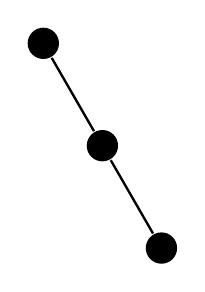
\begin{tikzpicture}
        [level distance=13mm,
        every node/.style={circle,inner sep=4pt, thick},
        ]
        \node[fill=black] {}
          child[missing]
          child{node[fill=black] {}
            child[missing]
            child{node[fill=black] {}
              child[missing]
              child[missing]
            }
          };
      \end{tikzpicture}
    \end{center}
  \end{minipage}
  \begin{minipage}{0.32\textwidth}
    \begin{center}
      \small
      The best and worst case for black height relative to total height of the tree,
      respectively.

    \end{center}
  \end{minipage}
  \begin{minipage}{0.33\textwidth}
    \begin{center}
      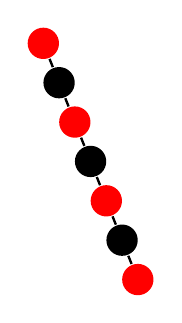
\begin{tikzpicture}
        [level distance=5mm,
        sibling distance=4mm,
        every node/.style={circle,inner sep=4pt, thick},
        ]
        \node[fill=red] {}
          child[missing]
          child{node[fill=black] {}
            child[missing]
            child{node[fill=red] {}
              child[missing]
              child{node[fill=black] {}
                child[missing]
                child{node[fill=red] {}
                  child[missing]
                  child{node[fill=black] {}
                    child[missing]
                    child{node[fill=red] {}
                      child[missing]
                      child[missing]
                    }
                  }
                }
              }
            }
          };
      \end{tikzpicture}
    \end{center}
  \end{minipage}
\end{frame}

\begin{frame}
  \frametitle{All Roads}

  \keyBox{}{This means on a given path to the bottom, there can be at worst approximately
  as many red nodes as there are black nodes.}

  \pause
  \vspace{\fill}

  Equivalently, any path from the root to the bottom can be at worst twice the
  length of another.

  \pause
  \vspace{\fill}

  This isn't a perfectly balanced tree, but it turns out this is close enough to guarantee
  asymptotic $O(\log n)$ traversal.

  \pause
  \vspace{\fill}

  That's the theory. How do we ensure that we can maintain these invariants?
\end{frame}

\sectionSlide{2}{Maintaining Invariants}

\begin{frame}
  \frametitle{Balance in All Things}

  The main operations we are concerned with are \code{insert} and \code{remove}. Since a
  red-black tree is a BST, we can look up in the same way, by just traversing down a path
  according to our comparison function.

  \pause
  \vspace{\fill}

  For insertion, we cannot avoid traversing the same path, as we cannot ever go to the
  left of a node we are \code{LESS} than, nor can we go right of a node we are
  \code{GREATER} than. However, \textit{after} we insert, we have some options for
  rebalancing our tree.

  \pause
  \vspace{\fill}

  \defBox{}{A \term{self-balancing tree} is a kind of tree data structure that can
  perform some balancing operations upon insertion or removal, to ensure the tree
  remains approximately balanced.}
\end{frame}

\begin{frame}
  \frametitle{The Color of Insertion}

  Let's consider the insertion case. If we're inserting into an arbitrary tree, what should
  we color the newly created node?

  \pause
  \vspace{\fill}

  \begin{center}
    \begin{minipage}{0.33\textwidth}
      \begin{adjustbox}{center}
        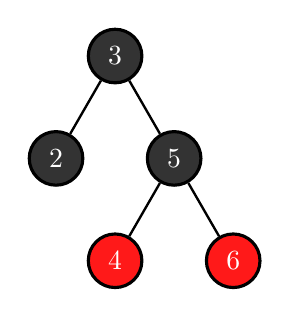
\begin{tikzpicture}
          \node[black] {3}
            child{node[black] {2}}
            child{node[black] {5}
              child{node[red] {4}}
              child{node[red] {6}}
            };
        \end{tikzpicture}
      \end{adjustbox}
    \end{minipage}
  \pause
    \begin{minipage}{0.15\textwidth}
      \begin{center}
        insert \code{1} $\mapsto$
      \end{center}
    \end{minipage}
    \begin{minipage}{0.33\textwidth}
        \begin{adjustbox}{center}
          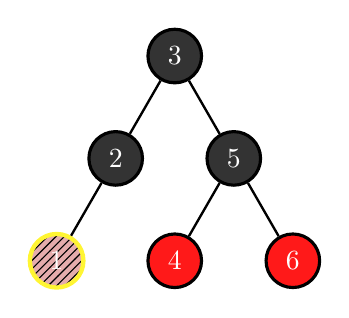
\begin{tikzpicture}
            \node[black] {3}
              child{node[black] {2}
                child{node[unknown, highlight] {1}
                }
                child[missing]
              }
              child{node[black] {5}
                child{node[red] {4}}
                child{node[red] {6}}
              };
          \end{tikzpicture}
        \end{adjustbox}
    \end{minipage}
  \end{center}

  \pause
  \vspace{\fill}

  Clearly, we have two cases. We can either color the node red, or we can color
  the node black.
\end{frame}

\begin{frame}
  \frametitle{Inserting: Black}

  Consider the black height invariant. If every path in the tree has the same black
  height, then clearly we cannot color the node black, because the newly created path
  will have a greater black height!

  \pause
  \vspace{\fill}

  \begin{center}
  \begin{minipage}{0.37\textwidth}
    \badbox{
      \node[black] (3) {3}
        child[highlight3]{node[black] {2}
          child[highlight3]{node[black, highlight] {1}
          }
          child[missing]
        }
        child{node[black] (5) {5}
          child{node[red] (4) {4}}
          child{node[red] {6}}
        };
        \draw[highlight2] (3) -- (5); % Specify the edge between nodes 3 and 5
        \draw[highlight2] (5) -- (4); % Specify the edge between nodes 3 and 5
    }{\xmark}{\cmark}
  \end{minipage}
  \hfill
  \pause
  \begin{minipage}{0.5\textwidth}
    \raggedright
    Black height ({\color{blue}blue path}): 3

    \pause
    \vspace{10pt}

    Black height ({\color{magenta} magenta path}): 2
  \end{minipage}
  \end{center}
\end{frame}

\begin{frame}
  \frametitle{Inserting: Red}

  What if we color the node red?

  \pause
  \vspace{\fill}

  \begin{center}
  \begin{minipage}{0.37\textwidth}
    \goodbox{
      \node[black] {3}
        child{node[black] {2}
          child{node[red, highlight] {1}
          }
          child[missing]
        }
        child{node[black] {5}
          child{node[red] {4}}
          child{node[red] {6}}
        };
    }{}
  \end{minipage}
  \hfill
  \pause
  \begin{minipage}{0.6\textwidth}
    \raggedright
    We see that coloring a node red will \textbf{always} end up satisfying the
    black height invariant, because the black height of every path will
    remain the same.

    \pause
    \vspace{20pt}

    But, what about our other invariants? Let's see an example on a
    slightly different tree.
  \end{minipage}
  \end{center}
\end{frame}

\begin{frame}
  \frametitle{An Insertion Example}

  Let's insert again on a different tree. This time, suppose we're inserting
  with a key of \code{2}.

  \pause
  \vspace{\fill}

  \begin{center}
    \begin{minipage}{0.33\textwidth}
      \begin{adjustbox}{center}
        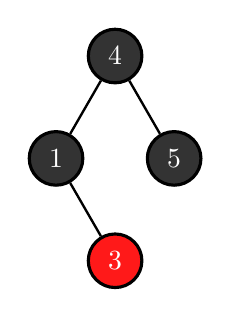
\begin{tikzpicture}
          \node[black] {4}
            child{node[black] {1}
              child[missing]
              child{node[red]{3}}
            }
            child{node[black] {5}};
        \end{tikzpicture}
      \end{adjustbox}
    \end{minipage}
    \pause
    \begin{minipage}{0.15\textwidth}
      \begin{center}
        insert \code{2} $\mapsto$
      \end{center}
    \end{minipage}
    \begin{minipage}{0.33\textwidth}
        \begin{adjustbox}{center}
          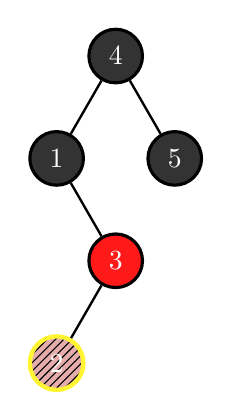
\begin{tikzpicture}
            \node[black] {4}
              child{node[black] {1}
                child[missing]
                child{node[red]{3}
                  child{node[unknown, highlight]{2}}
                  child[missing]
                }
              }
              child{node[black] {5}};
          \end{tikzpicture}
        \end{adjustbox}
    \end{minipage}
  \end{center}

  \pause
  \vspace{\fill}

  As before, let's color the node red.
\end{frame}

\begin{frame}
  \frametitle{Red-Red Violations}

  \begin{center}
  \begin{minipage}{0.37\textwidth}
    \badbox{
      \node[black] {4}
        child{node[black] {1}
          child[missing]
          child{node[red] (p) {3}
            child{node[red, highlight] (c) {2}}
            child[missing]
          }
        }
        child{node[black] {5}};
      \draw[rr] (p) -- (c);
    }{\cmark}{\xmark}
  \end{minipage}
  \pause
  \hfill
  \begin{minipage}{0.6\textwidth}
    \raggedright

    Uh oh, our heuristic of "always color new nodes red" didn't get us
    very far.

    \vspace{10pt}

    It only works in the case where our parent is black. Otherwise, we end
    up in a \term{red-red violation}.

    \pause
    \vspace{10pt}

    We also probably don't want to produce a tree of this shape anyways,
    because it's not as balanced as it could be! How can we fix this?

  \end{minipage}
  \end{center}
\end{frame}

\begin{frame}
  \frametitle{An Ideal Tree}

  \begin{center}
  \begin{minipage}{0.6\textwidth}
    \raggedright

    If we had free rein to transform this tree, how would we ideally balance it?

    \pause
    \vspace{10pt}

    We would like to produce this tree:

    \pause
    \vspace{20pt}

    But what should we color the nodes of
    \tikz[inline] \node[textnode]{\code{1}};,
    \tikz[inline] \node[textnode]{\code{2}};, and
    \tikz[inline] \node[textnode]{\code{3}};
    to ensure our invariants are respected?

    \vspace{20pt}

    We are going to choose to color the higher node \colr{red}, which will force
    its children to be \colb{black}, and see why this was the correct choice.
  \end{minipage}
  \hfill
  \begin{minipage}{0.37\textwidth}
      \centering

        \only<3->{
        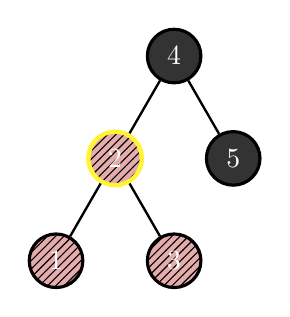
\begin{tikzpicture}
          \node[black] {4}
            child{node[unknown, highlight] {2}
              child{node[unknown] {1}}
              child{node[unknown] {3}}
            }
            child{node[black] {5}};
        \end{tikzpicture}
        }
  \end{minipage}
  \end{center}
\end{frame}

\begin{frame}
  \frametitle{Triads of Color}

  \begin{center}
  \begin{minipage}{0.6\textwidth}
    \raggedright

    This will end up producing a valid red-black tree.

    \vspace{10pt}

    But why did we choose to do it this way? We could have
    also decided to color it the other way, with the root
    node being black, and the children being red.

  \end{minipage}
  \hfill
  \begin{minipage}{0.37\textwidth}
    \goodbox{
          \node[black] {4}
            child{node[red, highlight] {2}
              child{node[black, highlight] {1}}
              child{node[black, highlight] {3}}
            }
            child{node[black] {5}};
    }{}
  \end{minipage}
  \end{center}
\end{frame}

\begin{frame}
  \frametitle{Triads of Color}

  \begin{center}
  \begin{minipage}{0.6\textwidth}
    \raggedright

    This is a valid red-black tree, but we will see that there
    are cases where we can't do this!

  \end{minipage}
  \hfill
  \begin{minipage}{0.37\textwidth}

    \goodbox{
      \node[black] {4}
        child{node[black, highlight] {2}
          child{node[red, highlight] {1}}
          child{node[red, highlight] {3}}
        }
        child{node[black] {5}};
    }{}
  \end{minipage}
  \end{center}
\end{frame}

\begin{frame}
  \frametitle{Another Insertion Example}

  Let's insert again on a tree which looks very similar, but has an extra
  \code{0} node. As before, we insert the key \code{2}:

    \pause
  \vspace{\fill}

  \begin{center}
    \begin{minipage}{0.33\textwidth}
      \begin{adjustbox}{center}
        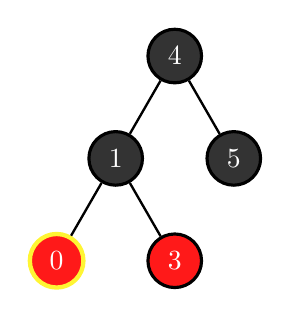
\begin{tikzpicture}
          \node[black] {4}
            child{node[black] {1}
              child{node[red, highlight]{0}}
              child{node[red]{3}}
            }
            child{node[black] {5}};
        \end{tikzpicture}
      \end{adjustbox}
    \end{minipage}
    \pause
    \begin{minipage}{0.15\textwidth}
      \begin{center}
        insert \code{2} $\mapsto$
      \end{center}
    \end{minipage}
    \begin{minipage}{0.33\textwidth}
        \begin{adjustbox}{center}
          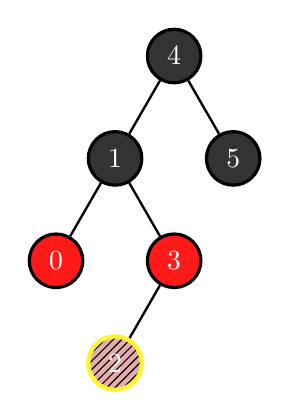
\begin{tikzpicture}
            \node[black] {4}
              child{node[black] {1}
                child{node[red]{0}}
                child{node[red]{3}
                  child{node[unknown, highlight]{2}}
                  child[missing]
                }
              }
              child{node[black] {5}};
          \end{tikzpicture}
        \end{adjustbox}
    \end{minipage}
  \end{center}
\end{frame}

\begin{frame}
  \frametitle{Another Insertion Example}

  \begin{center}
  \begin{minipage}{0.6\textwidth}
    \raggedright

    Well, if we want to rebalance this tree in the same way, we have to
    move the \code{2} up to \code{1}'s current position. But what should we
    do with the \code{0} node?

    \pause
    \vspace{10pt}

    Because \code{0} is less than \code{1}, we have no choice but to keep it
    left of \code{1}! So we get:

    \pause
    \vspace{10pt}

    Now, we have two choices over what we can color this triplet.

  \end{minipage}
  \hfill
  \begin{minipage}{0.37\textwidth}
    \centering
    \only<3->{
    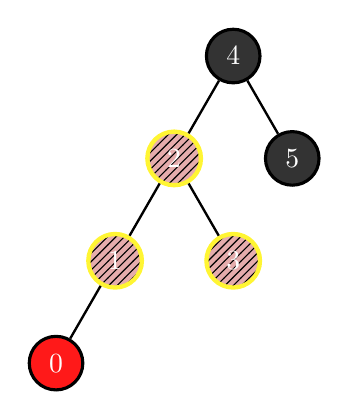
\begin{tikzpicture}
      \node[black] {4}
        child{node[unknown, highlight] {2}
          child{node[unknown, highlight] (p) {1}
            child{node[red] (c) {0}}
            child[missing]
          }
          child{node[unknown, highlight] {3}}
        }
        child{node[black] {5}};
    \end{tikzpicture}
    }
  \end{minipage}
  \end{center}
\end{frame}

\begin{frame}
  \frametitle{Canonical Red Roots}

  \begin{center}
  \begin{minipage}{0.37\textwidth}
    \badbox{
      \node[black] {4}
        child{node[black, highlight] {2}
          child{node[red, highlight] (p) {1}
            child{node[red] (c) {0}}
            child[missing]
          }
          child{node[red, highlight] {3}}
        }
        child{node[black] {5}};
        \draw[rr] (p) -- (c);
    }{\cmark}{\xmark}

  \end{minipage}
  \hfill
  \begin{minipage}{0.2\textwidth}
    \raggedright

    We see that only the triplet coloring with red at the root
    is valid!

    \vspace{10pt}

    This will form the basis for our canonical rebalance coloring
    scheme.
  \end{minipage}
  \hfill
  \begin{minipage}{0.37\textwidth}
    \goodbox{
      \node[black] {4}
        child{node[red, highlight] {2}
          child{node[black, highlight] {1}
            child{node[red] {0}}
            child[missing]
          }
          child{node[black, highlight] {3}}
        }
        child{node[black] {5}};
    }{}
  \end{minipage}
  \end{center}
\end{frame}

\begin{frame}
  \frametitle{Kinds of Rotations}

  Now that we've seen a few examples, we're ready to more in-depth describe our
  scheme for inserting nodes into a red-black tree.

  \pause
  \vspace{\fill}

  Our idea will be to insert a node, and always color it red, to maintain
  black height. If this induces a red-red violation, then we will simply rotate
  the tree, and recolor to prevent a red-red violation.
\end{frame}

\begin{frame}
  \frametitle{Kinds of Rotations}

  There are four cases we are interested in, for red-red violations.

  \pause
  \vspace{\fill}

  \begin{center}
    \begin{minipage}{0.24\textwidth}
      \centering
      \begin{tikzpicture}[scale=0.8]
        \node[black] {z}
          child{node[red] {\small y}
            child{node[red] {x}
              child{node[subtree] {\contour{black}{1}}}
              child{node[subtree] {\contour{black}{2}}}
            }
            child{node[subtree] {\contour{black}{3}}}
          }
          child{node[subtree] {\contour{black}{4}}};
      \end{tikzpicture}
    \end{minipage}
    \hfill\vline\hfill
    \pause
    \begin{minipage}{0.24\textwidth}
      \centering
      \begin{tikzpicture}[scale=0.8]
        \node[black] {z}
          child{node[red] {x}
            child{node[subtree] {\contour{black}{1}}}
            child{node[red] {\small y}
              child{node[subtree] {\contour{black}{2}}}
              child{node[subtree] {\contour{black}{3}}}
            }
          }
          child{node[subtree] {\contour{black}{4}}};
      \end{tikzpicture}
    \end{minipage}
    \hfill\vline\hfill
    \pause
    \begin{minipage}{0.24\textwidth}
      \centering
      \begin{tikzpicture}[scale=0.8]
        \node[black] {x}
          child{node[subtree]{\contour{black}{1}}}
          child{node[red] {z}
            child{node[red] {\small y}
              child{node[subtree]{\contour{black}{2}}}
              child{node[subtree]{\contour{black}{3}}}
            }
            child{node[subtree]{\contour{black}{4}}}
          };
      \end{tikzpicture}
    \end{minipage}
    \hfill\vline\hfill
    \pause
    \begin{minipage}{0.24\textwidth}
      \centering
      \begin{tikzpicture}[scale=0.8]
        \node[black] {x}
          child{node[subtree] {\contour{black}{1}}}
          child{node[red] {\small y}
            child{node[subtree] {\contour{black}{2}}}
            child{node[red] {z}
              child{node[subtree] {\contour{black}{3}}}
              child{node[subtree] {\contour{black}{4}}}
            }
          };
      \end{tikzpicture}
    \end{minipage}
  \end{center}

  \pause
  \vspace{\fill}

  Given three nodes with arbitrary children, it turns out there is a
  prescribed way that we will rotate each of these cases. In fact,
  the resulting subtree is the same!
\end{frame}

\begin{frame}
  \frametitle{A Rebalancing Target}

  \begin{center}
    \begin{minipage}{0.58\textwidth}
      \raggedright

      Given nodes \code{x}, \code{y}, and \code{z}, which are ordered in the
      same way as the letters we have used to denote them, there is only one
      tree which we can produce:

      \pause
      \vspace{10pt}

      A key observation of this rebalancing scheme is that, because the
      bottom nodes are colored black, it is \textbf{impossible} to produce a red-red
      violation from the connections to the children trees \code{1}, \code{2},
      \code{3}, and \code{4}, irrespective of color!

      \vspace{10pt}

      Given that we have also preserved black height, because each path to
      the children trees still encounters one black node, are we done?
    \end{minipage}
    \hfill
    \begin{minipage}{0.4\textwidth}
      \centering
      \only<2->{
      \begin{tikzpicture}[scale=1.2,
        level 1/.style={sibling distance=2cm},
        level 2/.style={sibling distance=1cm},
        ]
        \node[red] {\small y}
          child{node[black] {x}
            child{node[subtree] {\contour{black}{1}}}
            child{node[subtree] {\contour{black}{2}}}
          }
          child{node[black] {z}
            child{node[subtree] {\contour{black}{3}}}
            child{node[subtree] {\contour{black}{4}}}
          };
      \end{tikzpicture}
      }
    \end{minipage}
  \end{center}
\end{frame}

\begin{frame}
  \frametitle{Right Rotations}

  \begin{center}
    \begin{minipage}{0.25\textwidth}
      \centering
      \begin{tikzpicture}[scale=0.8]
        \node[black] {z}
          child{node[red] {\small y}
            child{node[red] {x}
              child{node[subtree] {\contour{black}{1}}}
              child{node[subtree] {\contour{black}{2}}}
            }
            child{node[subtree] {\contour{black}{3}}}
          }
          child{node[subtree] {\contour{black}{4}}};
      \end{tikzpicture}
    \end{minipage}
    \hfill
    \begin{minipage}{0.07\textwidth}
      \centering
      \large$\longmapsto$
    \end{minipage}
    \hfill
    \begin{minipage}{0.3\textwidth}
      \centering
      \begin{tikzpicture}[scale=1.2,
        level 1/.style={sibling distance=2cm},
        level 2/.style={sibling distance=1cm},
        ]
        \node[red] {\small y}
          child{node[black] {x}
            child{node[subtree] {\contour{black}{1}}}
            child{node[subtree] {\contour{black}{2}}}
          }
          child{node[black] {z}
            child{node[subtree] {\contour{black}{3}}}
            child{node[subtree] {\contour{black}{4}}}
          };
      \end{tikzpicture}
    \end{minipage}
    \hfill
    \begin{minipage}{0.07\textwidth}
      \centering
      \large$\longmapsfrom$
    \end{minipage}
    \hfill
    \begin{minipage}{0.25\textwidth}
      \centering
      \begin{tikzpicture}[scale=0.8]
        \node[black] {z}
          child{node[red] {x}
            child{node[subtree] {\contour{black}{1}}}
            child{node[red] {\small y}
              child{node[subtree] {\contour{black}{2}}}
              child{node[subtree] {\contour{black}{3}}}
            }
          }
          child{node[subtree] {\contour{black}{4}}};
      \end{tikzpicture}
    \end{minipage}
  \end{center}

  \pause
  \vspace{\fill}

  These two examples illustrate what is known as a \term{right rotation}. We
  will implement a function \code{restoreLeft} to do this, because it's
  restoring a path that goes left.
\end{frame}


\begin{frame}
  \frametitle{Left Rotations}

  \begin{center}
    \begin{minipage}{0.25\textwidth}
      \centering
      \begin{tikzpicture}[scale=0.8]
        \node[black] {x}
          child{node[subtree]{\contour{black}{1}}}
          child{node[red] {z}
            child{node[red] {\small y}
              child{node[subtree]{\contour{black}{2}}}
              child{node[subtree]{\contour{black}{3}}}
            }
            child{node[subtree]{\contour{black}{4}}}
          };
      \end{tikzpicture}
    \end{minipage}
    \begin{minipage}{0.07\textwidth}
      \centering
      \large$\longmapsto$
    \end{minipage}
    \begin{minipage}{0.3\textwidth}
      \centering
      \begin{tikzpicture}[scale=1.2,
        level 1/.style={sibling distance=2cm},
        level 2/.style={sibling distance=1cm},
        ]
        \node[red] {\small y}
          child{node[black] {x}
            child{node[subtree] {\contour{black}{1}}}
            child{node[subtree] {\contour{black}{2}}}
          }
          child{node[black] {z}
            child{node[subtree] {\contour{black}{3}}}
            child{node[subtree] {\contour{black}{4}}}
          };
      \end{tikzpicture}
    \end{minipage}
    \begin{minipage}{0.07\textwidth}
      \centering
      \large$\longmapsfrom$
    \end{minipage}
    \begin{minipage}{0.25\textwidth}
      \centering
      \begin{tikzpicture}[scale=0.8]
        \node[black] {x}
          child{node[subtree] {\contour{black}{1}}}
          child{node[red] {\small y}
            child{node[subtree] {\contour{black}{2}}}
            child{node[red] {z}
              child{node[subtree] {\contour{black}{3}}}
              child{node[subtree] {\contour{black}{4}}}
            }
          };
      \end{tikzpicture}
    \end{minipage}
  \end{center}

  \pause
  \vspace{\fill}

  These two examples illustrate what is known as a \term{left rotation}. Similarly,
  we will implement a function called \code{restoreRight} that will fix this
  situation.
\end{frame}

\begin{frame}
  \frametitle{Another Another Insertion Example}

  Let's see! Let's do another example, which is identical to the last one, except
  that the root is colored red. As before, we insert the key \code{2}:

  \pause
  \vspace{\fill}

  \begin{center}
    \begin{minipage}{0.25\textwidth}
      \begin{adjustbox}{center}
        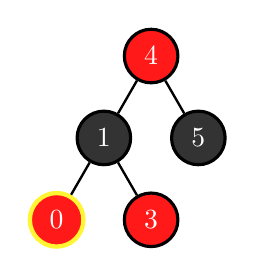
\begin{tikzpicture}[scale=0.8]
          \node[red] {4}
            child{node[black] {1}
              child{node[red, highlight]{0}}
              child{node[red]{3}}
            }
            child{node[black] {5}};
        \end{tikzpicture}
      \end{adjustbox}
    \end{minipage}
  \pause
    \begin{minipage}{0.10\textwidth}
      \begin{center}
        insert \code{2} $\mapsto$
      \end{center}
    \end{minipage}
    \begin{minipage}{0.25\textwidth}
        \begin{adjustbox}{center}
          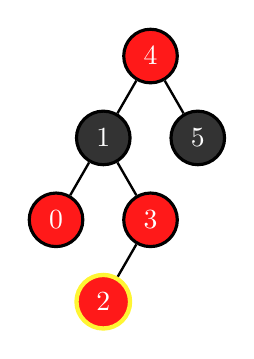
\begin{tikzpicture}[scale=0.8]
            \node[red] {4}
              child{node[black] {1}
                child{node[red]{0}}
                child{node[red]{3}
                  child{node[red, highlight]{2}}
                  child[missing]
                }
              }
              child{node[black] {5}};
          \end{tikzpicture}
        \end{adjustbox}
    \end{minipage}
  \pause
    \begin{minipage}{0.10\textwidth}
      \begin{center}
        rebalance! $\mapsto$
      \end{center}
    \end{minipage}
    \begin{minipage}{0.25\textwidth}
        \begin{adjustbox}{center}
          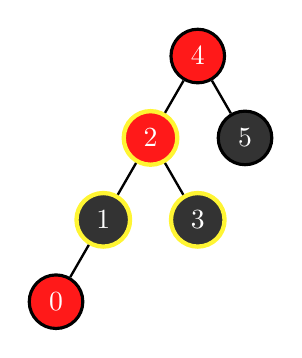
\begin{tikzpicture}[scale=0.8]
            \node[red] {4}
              child{node[red, highlight] {2}
                child{node[black, highlight]{1}
                  child{node[red]{0}}
                  child[missing]
                }
                child{node[black, highlight]{3}}
              }
              child{node[black] {5}};
          \end{tikzpicture}
        \end{adjustbox}
    \end{minipage}
  \end{center}

  \pause
  \vspace{\fill}

  Uh oh...
\end{frame}

\begin{frame}
  \frametitle{Another Another Insertion Example}

  \begin{center}
    \begin{minipage}{0.37\textwidth}
      \badbox{
        \node[red] (p) {4}
          child{node[red] (c) {2}
            child{node[black]{1}
              child{node[red]{0}}
              child[missing]
            }
            child{node[black]{3}}
          }
          child{node[black] {5}};
        \draw[rr] (p) -- (c);
      }{\cmark}{\xmark}
    \end{minipage}
    \hfill
    \begin{minipage}{0.6\textwidth}
      \raggedright

      We see that we end up with a red-red violation.

      \pause
      \vspace{10pt}

      However, a neat fact about red-black trees is that the
      root can always be colored black, no matter what!

      \pause
      \vspace{10pt}

      \customBox{Check your understanding}{\, Why does this
      preserve the invariants?}
    \end{minipage}
  \end{center}
\end{frame}

\begin{frame}
  \frametitle{On Preserving Balance}

  \begin{center}
    \begin{minipage}{0.37\textwidth}
      \goodbox{
        \node[black, highlight] (p) {4}
          child{node[red] (c) {2}
            child{node[black]{1}
              child{node[red]{0}}
              child[missing]
            }
            child{node[black]{3}}
          }
          child{node[black] {5}};
      }{}
    \end{minipage}
    \hfill
    \begin{minipage}{0.6\textwidth}
      \raggedright

      So by coloring the root node black for free, we end up
      getting a valid red-black tree.

      \pause
      \vspace{10pt}

      A question remains -- did we get lucky? What happens if we
      aren't at the root?

      \pause
      \vspace{10pt}

      Our issue was that rebalancing our subtree to get rid of a
      red-red violation might introduce another red-red violation,
      slightly above it. Our scheme will be to \textbf{continuously rebalance},
      and push the red-red violation further upwards, until we potentially
      reach the root, or no longer have a violation.

    \end{minipage}
  \end{center}
\end{frame}

\quizBreak{DICHROMATIC}

\sectionSlide{3}{Implementing Red-Black Trees}

\begin{frame}
  \frametitle{Almost Done}

  We can formalize the notion of our algorithm by defining a new kind of
  tree, which we will call an \term{almost red-black tree}.\footnote{
    Sort of in the same way that I am an \textit{almost professor},
    which is to say, I am not one.
  }

  \pause
  \vspace{\fill}

  \defBox{}{An \term{almost red-black tree} shares the same properties
  as a red-black tree, but its root node and one of the root node's children
  may both be red.}

  \pause
  \vspace{\fill}

  In other words, an almost red-black tree is allowed to break the red children
  invariant, once, and only at the root.
\end{frame}

\begin{frame}
  \frametitle{Restoration Functions}

  Here is a specification for our rotation functions, which we will call
  \code{restoreLeft} and \code{restoreRight}.

  \pause
  \spec
    {restoreLeft}
    {'a rbtree -> 'a rbtree}
    {\code{T} is an RBT, or \code{T} is a \code{Black} tree, with a \textbf{left}
    child that is an ARBT, and a right child that is an RBT}
    {\code{restoreLeft T} is an RBT with the same entries as \code{T}}

  \pause
  \spec
    {restoreRight}
    {'a rbtree -> 'a rbtree}
    {\code{T} is an RBT, or \code{T} is a \code{Black} tree, with a \textbf{right}
    child that is an ARBT, and a left child that is an RBT}
    {\code{restoreRight T} is an RBT with the same entries as \code{T}}
\end{frame}

\begin{frame}
  \frametitle{Restoration Functions}

  Recall that functions which do not appear in the signature of a module
  are not visible to users of the library. This means that, after we
  write \code{restoreLeft} and \code{restoreRight}, they are only for
  internal use, in helping us implement \code{insert}!

  \pause
  \vspace{\fill}

  Note also that although \code{restoreLeft} and \code{restoreRight} produce
  true RBTs, it may produce an ARBT in the node right above it, if it is
  colored red. We will percolate these fixes up as we insert, however.
\end{frame}


\begin{frame}[fragile]
  \frametitle{Restoring Left}

  \begin{codeblock}
    fun restoreLeft <b(<blBlackbl>(<rRedr>(<rRedr>(t1,x,t2),y,t3),z,t4))b> =
      <b<rRedr>(<blBlackbl>(t1,x,t2), y, <blBlackbl>(t3,z,t4))b>
  \end{codeblock}

  \pause
  \begin{center}
    \begin{minipage}{0.35\textwidth}
      \centering
      \begin{tikzpicture}[scale=0.8]
        \node[black] {z}
          child{node[red] {\small y}
            child{node[red] {x}
              child{node[subtree] {\contour{black}{1}}}
              child{node[subtree] {\contour{black}{2}}}
            }
            child{node[subtree] {\contour{black}{3}}}
          }
          child{node[subtree] {\contour{black}{4}}};
      \end{tikzpicture}
    \end{minipage}
    \pause
    \begin{minipage}{0.1\textwidth}
      \centering
      \large$\longmapsto$
    \end{minipage}
    \begin{minipage}{0.35\textwidth}
      \centering
      \begin{tikzpicture}[scale=1.2,
        level 1/.style={sibling distance=2cm},
        level 2/.style={sibling distance=1cm},
        ]
        \node[red] {\small y}
          child{node[black] {x}
            child{node[subtree] {\contour{black}{1}}}
            child{node[subtree] {\contour{black}{2}}}
          }
          child{node[black] {z}
            child{node[subtree] {\contour{black}{3}}}
            child{node[subtree] {\contour{black}{4}}}
          };
      \end{tikzpicture}
    \end{minipage}
  \end{center}
\end{frame}

\begin{frame}[fragile]
  \frametitle{Restoring Left}

  \begin{codeblock}
    fun restoreLeft <b(<blBlackbl>(<rRedr>(<rRedr>(t1,x,t2),y,t3),z,t4))b> =
          <b<rRedr>(<blBlackbl>(t1,x,t2), y, <blBlackbl>(t3,z,t4))b>
      | restoreLeft <b(<blBlackbl>(<rRedr>(t1,x,<rRedr>(t2,y,t3)),z,t4))b> =
          <b<rRedr>(<blBlackbl>(t1,x,t2), y, <blBlackbl>(t3,z,t4))b>
  \end{codeblock}

  \pause
  \begin{center}
    \begin{minipage}{0.35\textwidth}
      \centering
      \begin{tikzpicture}[scale=0.8]
        \node[black] {z}
          child{node[red] {x}
            child{node[subtree] {\contour{black}{1}}}
            child{node[red] {\small y}
              child{node[subtree] {\contour{black}{2}}}
              child{node[subtree] {\contour{black}{3}}}
            }
          }
          child{node[subtree] {\contour{black}{4}}};
      \end{tikzpicture}
    \end{minipage}
    \pause
    \begin{minipage}{0.1\textwidth}
      \centering
      \large$\longmapsto$
    \end{minipage}
    \begin{minipage}{0.35\textwidth}
      \centering
      \begin{tikzpicture}[scale=1.2,
        level 1/.style={sibling distance=2cm},
        level 2/.style={sibling distance=1cm},
        ]
        \node[red] {\small y}
          child{node[black] {x}
            child{node[subtree] {\contour{black}{1}}}
            child{node[subtree] {\contour{black}{2}}}
          }
          child{node[black] {z}
            child{node[subtree] {\contour{black}{3}}}
            child{node[subtree] {\contour{black}{4}}}
          };
      \end{tikzpicture}
    \end{minipage}
  \end{center}
\end{frame}

\begin{frame}[fragile]
  \frametitle{Restoring Left}

  \begin{codeblock}
    fun restoreLeft <b(<blBlackbl>(<rRedr>(<rRedr>(t1,x,t2),y,t3),z,t4))b> =
          <b<rRedr>(<blBlackbl>(t1,x,t2), y, <blBlackbl>(t3,z,t4))b>
      | restoreLeft <b(<blBlackbl>(<rRedr>(t1,x,<rRedr>(t2,y,t3)),z,t4))b> =
          <b<rRedr>(<blBlackbl>(t1,x,t2), y, <blBlackbl>(t3,z,t4))b>
      | restoreLeft other = other
  \end{codeblock}

  \pause
  \vspace{\fill}

  And finally, any other input doesn't need to be restored from the left,
  so we omit it here.

  \vspace{\fill}

  Now we can proceed to the right case.
\end{frame}

\begin{frame}[fragile]
  \frametitle{Restoring Right}

  \begin{codeblock}
    fun restoreRight <b(<blBlackbl>(t1,x,<rRedr>(<rRedr>(t2,y,t3),z,t4)))b> =
          <b<rRedr>(<blBlackbl>(t1,x,t2), y, <blBlackbl>(t3,z,t4))b>
  \end{codeblock}

  \pause
  \begin{center}
    \begin{minipage}{0.35\textwidth}
      \centering
      \begin{tikzpicture}[scale=0.8]
        \node[black] {x}
          child{node[subtree]{\contour{black}{1}}}
          child{node[red] {z}
            child{node[red] {\small y}
              child{node[subtree]{\contour{black}{2}}}
              child{node[subtree]{\contour{black}{3}}}
            }
            child{node[subtree]{\contour{black}{4}}}
          };
      \end{tikzpicture}
    \end{minipage}
    \pause
    \begin{minipage}{0.1\textwidth}
      \centering
      \large$\longmapsto$
    \end{minipage}
    \begin{minipage}{0.35\textwidth}
      \centering
      \begin{tikzpicture}[scale=1.2,
        level 1/.style={sibling distance=2cm},
        level 2/.style={sibling distance=1cm},
        ]
        \node[red] {\small y}
          child{node[black] {x}
            child{node[subtree] {\contour{black}{1}}}
            child{node[subtree] {\contour{black}{2}}}
          }
          child{node[black] {z}
            child{node[subtree] {\contour{black}{3}}}
            child{node[subtree] {\contour{black}{4}}}
          };
      \end{tikzpicture}
    \end{minipage}
  \end{center}
\end{frame}

\begin{frame}[fragile]
  \frametitle{Restoring Right}

  \begin{codeblock}
    fun restoreRight <b(<blBlackbl>(t1,x,<rRedr>(<rRedr>(t2,y,t3),z,t4)))b> =
          <b<rRedr>(<blBlackbl>(t1,x,t2), y, <blBlackbl>(t3,z,t4))b>
      | restoreRight <b(<blBlackbl>(t1,x,<rRedr>(t2,y,<rRedr>(t3,z,t4))))b> =
          <b<rRedr>(<blBlackbl>(t1,x,t2), y, <blBlackbl>(t3,z,t4))b>
  \end{codeblock}

  \pause
  \begin{center}
    \begin{minipage}{0.35\textwidth}
      \centering
      \begin{tikzpicture}[scale=0.8]
        \node[black] {x}
          child{node[subtree] {\contour{black}{1}}}
          child{node[red] {\small y}
            child{node[subtree] {\contour{black}{2}}}
            child{node[red] {z}
              child{node[subtree] {\contour{black}{3}}}
              child{node[subtree] {\contour{black}{4}}}
            }
          };
      \end{tikzpicture}
    \end{minipage}
    \pause
    \begin{minipage}{0.1\textwidth}
      \centering
      \large$\longmapsto$
    \end{minipage}
    \begin{minipage}{0.35\textwidth}
      \centering
      \begin{tikzpicture}[scale=1.2,
        level 1/.style={sibling distance=2cm},
        level 2/.style={sibling distance=1cm},
        ]
        \node[red] {\small y}
          child{node[black] {x}
            child{node[subtree] {\contour{black}{1}}}
            child{node[subtree] {\contour{black}{2}}}
          }
          child{node[black] {z}
            child{node[subtree] {\contour{black}{3}}}
            child{node[subtree] {\contour{black}{4}}}
          };
      \end{tikzpicture}
    \end{minipage}
  \end{center}
\end{frame}

\begin{frame}[fragile]
  \frametitle{Restoring Right}

  \begin{codeblock}
    fun restoreRight <b(<blBlackbl>(t1,x,<rRedr>(<rRedr>(t2,y,t3),z,t4)))b> =
          <b<rRedr>(<blBlackbl>(t1,x,t2), y, <blBlackbl>(t3,z,t4))b>
      | restoreRight <b(<blBlackbl>(t1,x,<rRedr>(t2,y,<rRedr>(t3,z,t4))))b> =
          <b<rRedr>(<blBlackbl>(t1,x,t2), y, <blBlackbl>(t3,z,t4))b>
      | restoreRight other = other
  \end{codeblock}

  \pause
  \vspace{\fill}

  And finally, as before, \code{restoreRight} also acts as the identity function
  on any input which is not one of the two rotation cases.
\end{frame}


\begin{frame}[fragile]
  \frametitle{On to Insertion}

  Now that we've written our balancing functions, let's handle insertion.

  \pause
  \vspace{\fill}

  We will achieve this via two functions. One will carry out the
  insertion algorithm we described previously, and one will be a wrapper
  function that simply takes care of the rectifying any red-red violations
  at the root.
\end{frame}



\begin{frame}
  \frametitle{Does Anyone Read These Titles}

  \spec
    {insert}
    {(Key.t * 'a) -> 'a rbtree -> 'a rbtree}
    {\code{T} is an RBT}
    {\code{insert (k, v) T} is an RBT with all the entries of \code{T},
    plus the key-value pair \code{(k, v)}. If an entry already exists,
    it is replaced.}

  \pause
  \vspace{\fill}

  We will define the \code{ins} function locally to the definition of
  \code{insert}, meaning that it does not need to take the key-value
  pair as an argument, since it is already in the environment.

  \pause
  \vspace{\fill}

  \spec
    {ins}
    {'a rbtree -> 'a rbtree}
    {\code{T} is an RBT}
    {\code{ins (k, v) T} has the same specification as \code{insert}, but
    \code{ins (k, v) (Black v)} is an RBT, and \code{ins (k, v) (Red v)} is
    an ARBT.}
\end{frame}

\begin{frame}[fragile]
  \frametitle{Implementing \code{insert}}

  \begin{codeblock}
    fun insert (k, v) T =
      let
        fun ins T = (* ... *)
      in
        case ins (k, v) T of
          Red v => Black v
        | other => other
      end
  \end{codeblock}

  \pause
  \vspace{\fill}

  If there is ever a red root, we can safely recolor it to black. We only
  want to do this at the true root of the tree, however, hence why we have the
  outer \code{insert}, which is not recursive.

  \pause
  \vspace{\fill}

  Now, we must define the \code{ins} function, which will do the real work of
  the insertion algorithm.
\end{frame}

\begin{frame}[fragile]
  \frametitle{Implementing \code{ins}}

  Note that this function is being written in the body of \code{insert}, so
  we obtain the values of \code{k} and \code{v} as the argument, the
  key-value pair we are trying to insert.

  \pause
  \vspace{\fill}

  \begin{codeblock}
    fun ins Empty = Red (Empty, e, Empty)
      | ins (Black (l, (k', v'), r)) =
          (case Key.compare (k, k') of
            EQUAL   => Black (l, (k, v), r))
          | LESS    => restoreLeft (Black (ins l, (k', v'), r))
          | GREATER => restoreRight (Black (l, (k', v'), ins r))
      | ins (Red (l, (k', v'), r)) =
          (case Key.compare (k, k') of
            EQUAL   => Red (l, (k, v), r)
          | LESS    => Red (ins l, (k', v'), r)
          | GREATER => Red (l, (k', v'), ins r))
  \end{codeblock}
\end{frame}

\begin{frame}[fragile]
  \frametitle{Implementing \code{ins}}

  {\small
  \begin{codeblock}
    fun ins Empty = Red (Empty, e, Empty)
      | ins (Black (l, (k', v'), r)) =
          (case Key.compare (k, k') of
            EQUAL   => Black (l, (k, v), r))
          | LESS    => `restoreLeft` (Black (ins l, (k', v'), r))
          | GREATER => `restoreRight` (Black (l, (k', v'), ins r))
      | ins (Red (l, (k', v'), r)) =
          (case Key.compare (k, k') of
            EQUAL   => Red (l, (k, v), r)
          | LESS    => Red (ins l, (k', v'), r)
          | GREATER => Red (l, (k', v'), ins r))
  \end{codeblock}
  }

  \pause
  \vspace{\fill}

  Note that we do the \code{restoreLeft} and \code{restoreRight} calls only
  when inserting into the left and right trees, respectively.

  \pause
  \vspace{\fill}

  We also don't need to restore when inserting into a \code{Red} tree --
  why is that?

\end{frame}

\begin{frame}[fragile]
  \frametitle{Lookup}

  Lookup for a red-black tree looks similar to the regular BST case:

  \pause
  \vspace{\fill}

  \begin{codeblock}
    fun lookup k Empty = NONE
      | lookup k ( Red (l, (k', v'), r)
                 | Black (l, (k', v'), r)) =
          case Key.compare (k, k') of
            EQUAL   => SOME v'
          | LESS    => lookup k l
          | GREATER => lookup k r
  \end{codeblock}

  \pause
  \vspace{\fill}

  Here, we make use of something called an \term{or-pattern}, to
  reduce some boilerplate. This is a pattern \code{(<pat1> | <pat2>)}
  that is matched if either \code{<pat1>} or \code{<pat2>} is matched, but
  is only valid so long as both patterns introduce the exact same bindings,
  with the same types.
\end{frame}

\begin{frame}[fragile]
  \frametitle{to err is human, to functor divine}

  Now we can assemble the final parts of the puzzle, by putting everything
  we just wrote in a functor\footnote{
    Remember those? This didn't stop being a lecture on modules,
    or anything.
  }, so that we can achieve full generality!

  \pause
  \vspace{\fill}

  \begin{codeblock}
    functor MkRedBlackDict (Key : ORD) :> POLY_DICT =
      struct
        structure Key = Key

        datatype 'a rbtree =
            Empty
          | Red of 'a rbtree * (Key.t * 'a) * 'a rbtree
          | Black of 'a rbtree * (Key.t * 'a) * 'a rbtree

        (* ... *)
      end
  \end{codeblock}
\end{frame}



\begin{frame}[fragile]
  \frametitle{The Final Implementation}

  \tiny

  \begin{codeblock}
    functor MkRedBlackDict (Key : ORD) :> POLY_DICT =
      struct
        structure Key = Key

        datatype 'a rbtree =
            Empty
          | Red of 'a rbtree * (Key.t * 'a) * 'a rbtree
          | Black of 'a rbtree * (Key.t * 'a) * 'a rbtree
        type 'a t = 'a rbtree

        val empty = Empty

        fun restoreLeft <b(<blBlackbl>(<rRedr>(<rRedr>(t1,x,t2),y,t3),z,t4))b> =
              <b<rRedr>(<blBlackbl>(t1,x,t2), y, <blBlackbl>(t3,z,t4))b>
          | restoreLeft <b(<blBlackbl>(<rRedr>(t1,x,<rRedr>(t2,y,t3)),z,t4))b> =
              <b<rRedr>(<blBlackbl>(t1,x,t2), y, <blBlackbl>(t3,z,t4))b>
          | restoreLeft other = other

        fun restoreRight <b(<blBlackbl>(t1,x,<rRedr>(<rRedr>(t2,y,t3),z,t4)))b> =
              <b<rRedr>(<blBlackbl>(t1,x,t2), y, <blBlackbl>(t3,z,t4))b>
          | restoreRight <b(<blBlackbl>(t1,x,<rRedr>(t2,y,<rRedr>(t3,z,t4))))b> =
              <b<rRedr>(<blBlackbl>(t1,x,t2), y, <blBlackbl>(t3,z,t4))b>
          | restoreRight other = other

        (* ... *)
  \end{codeblock}
\end{frame}

\begin{frame}[fragile]
  \frametitle{The Final Implementation}

  \tiny
  \begin{codeblock}
    (* ... *)

        fun insert (k, v) T =
          let
            fun ins Empty = Red (Empty, e, Empty)
              | ins (Black (l, (k', v'), r)) =
                  (case Key.compare (k, k') of
                    EQUAL   => Black (l, (k, v), r))
                  | LESS    => restoreLeft (Black (ins l, (k', v'), r))
                  | GREATER => restoreRight (Black (l, (k', v'), ins r))
              | ins (Red (l, (k', v'), r)) =
                  (case Key.compare (k, k') of
                    EQUAL   => Red (l, (k, v), r)
                  | LESS    => Red (ins l, (k', v'), r)
                  | GREATER => Red (l, (k', v'), ins r))
          in
            case ins (k, v) T of
              Red v => Black v
            | other => other
          end

        fun lookup k Empty = NONE
          | lookup k ( Red (l, (k', v'), r)
                     | Black (l, (k', v'), r)) =
              case Key.compare (k, k') of
                EQUAL   => SOME v'
              | LESS    => lookup k l
              | GREATER => lookup k r
      end
  \end{codeblock}
\end{frame}

\sectionSlide{4}{A Final Trace}

\begin{frame}[fragile]
  \frametitle{A Final Trace}

  \begin{center}
    \begin{minipage}{0.23\textwidth}
      \centering
      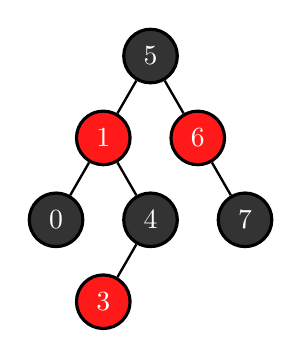
\begin{tikzpicture}[scale=0.8]
        \node[black] {5}
          child{node[red] {1}
            child{node[black]{0}}
            child{node[black]{4}
              child{node[red]{3}}
              child[missing]
            }
          }
          child{node[red] {6}
            child[missing]
            child{node[black]{7}}
          };
      \end{tikzpicture}
    \end{minipage}
    \hfill
    \pause
    \begin{minipage}{0.12\textwidth}
      \begin{center}
        insert \code{2} $\mapsto$
      \end{center}
    \end{minipage}
    \hfill
    \begin{minipage}{0.23\textwidth}
      \centering
      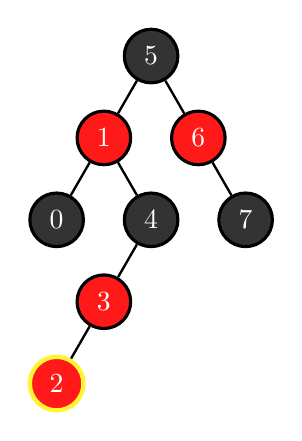
\begin{tikzpicture}[scale=0.8]
        \node[black] {5}
          child{node[red] {1}
            child{node[black]{0}}
            child{node[black]{4}
              child{node[red]{3}
                child{node[red, highlight]{2}}
                child[missing]
              }
              child[missing]
            }
          }
          child{node[red] {6}
            child[missing]
            child{node[black]{7}}
          };
      \end{tikzpicture}
    \end{minipage}
    \hfill
    \pause
    \begin{minipage}{0.12\textwidth}
      \begin{center}
        red-red violation! $\mapsto$
      \end{center}
    \end{minipage}
    \hfill
    \begin{minipage}{0.23\textwidth}
      \centering
      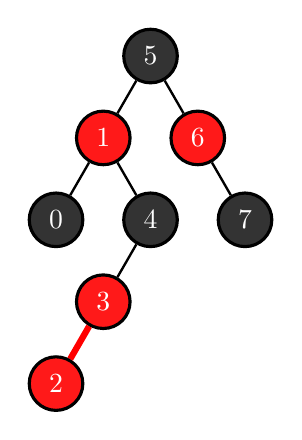
\begin{tikzpicture}[scale=0.8]
        \node[black] {5}
          child{node[red] {1}
            child{node[black]{0}}
            child{node[black]{4}
              child{node[red](p){3}
                child{node[red](c){2}}
                child[missing]
              }
              child[missing]
            }
          }
          child{node[red] {6}
            child[missing]
            child{node[black]{7}}
          };
        \draw[rr] (p) -- (c);
      \end{tikzpicture}
    \end{minipage}
  \end{center}
\end{frame}


\begin{frame}[fragile]
  \frametitle{A Final Trace}

  \begin{center}
    \begin{minipage}{0.23\textwidth}
      \centering
      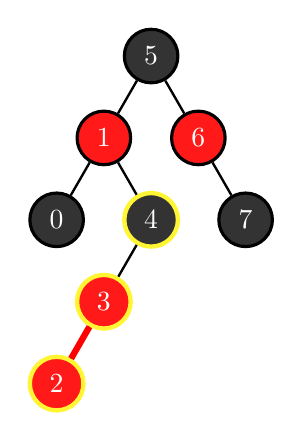
\begin{tikzpicture}[scale=0.8]
        \node[black] {5}
          child{node[red] {1}
            child{node[black]{0}}
            child{node[black, highlight]{4}
              child{node[red, highlight](p){3}
                child{node[red, highlight](c){2}}
                child[missing]
              }
              child[missing]
            }
          }
          child{node[red] {6}
            child[missing]
            child{node[black]{7}}
          };
        \draw[rr] (p) -- (c);
      \end{tikzpicture}
    \end{minipage}
    \hfill
    \pause
    \begin{minipage}{0.12\textwidth}
      \begin{center}
        rebalance! $\mapsto$
      \end{center}
    \end{minipage}
    \hfill
    \begin{minipage}{0.23\textwidth}
      \centering
      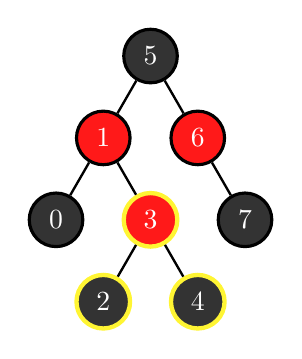
\begin{tikzpicture}[scale=0.8]
        \node[black] {5}
          child{node[red] {1}
            child{node[black]{0}}
            child{node[red, highlight]{3}
              child{node[black, highlight]{2}}
              child{node[black, highlight]{4}}
            }
          }
          child{node[red] {6}
            child[missing]
            child{node[black]{7}}
          };
      \end{tikzpicture}
    \end{minipage}
    \hfill
    \pause
    \begin{minipage}{0.12\textwidth}
      \begin{center}
        red-red violation! $\mapsto$
      \end{center}
    \end{minipage}
    \hfill
    \begin{minipage}{0.23\textwidth}
      \centering
      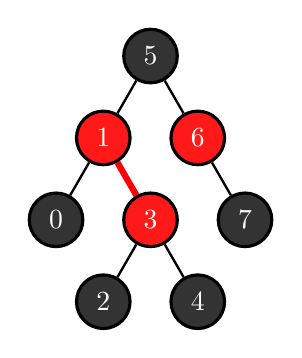
\begin{tikzpicture}[scale=0.8]
        \node[black] {5}
          child{node[red] (p) {1}
            child{node[black]{0}}
            child{node[red] (c) {3}
              child{node[black]{2}}
              child{node[black]{4}}
            }
          }
          child{node[red] {6}
            child[missing]
            child{node[black]{7}}
          };
        \draw[rr] (p) -- (c);
      \end{tikzpicture}
    \end{minipage}
  \end{center}
\end{frame}

\begin{frame}[fragile]
  \frametitle{A Final Trace}

  \begin{center}
    \begin{minipage}{0.30\textwidth}
      \centering
      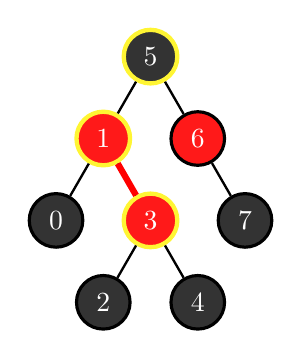
\begin{tikzpicture}[scale=0.8]
        \node[black, highlight] {5}
          child{node[red, highlight] (p) {1}
            child{node[black]{0}}
            child{node[red, highlight] (c) {3}
              child{node[black]{2}}
              child{node[black]{4}}
            }
          }
          child{node[red] {6}
            child[missing]
            child{node[black]{7}}
          };
        \draw[rr] (p) -- (c);
      \end{tikzpicture}
    \end{minipage}
    \pause
    \begin{minipage}{0.2\textwidth}
      \begin{center}
        rebalance! $\mapsto$
      \end{center}
    \end{minipage}
    \begin{minipage}{0.39\textwidth}
      \centering
      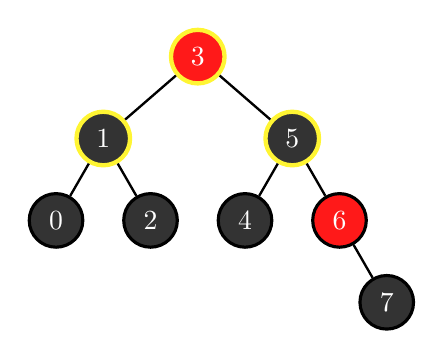
\begin{tikzpicture}[scale=0.8,
        level 1/.style={sibling distance=3cm},
        level 2/.style={sibling distance=1.5cm},
        ]
        \node[red, highlight] {3}
          child{node[black, highlight] {1}
            child{node[black] {0}}
            child{node[black] {2}}
          }
          child{node[black, highlight] {5}
            child{node[black] {4}}
            child{node[red] {6}
              child[missing]
              child{node[black] {7}}
            }
          };
      \end{tikzpicture}
    \end{minipage}
  \end{center}
\end{frame}

\begin{frame}[fragile]
  \frametitle{A Final Trace}

  \begin{center}
    \begin{minipage}{0.39\textwidth}
     \centering
      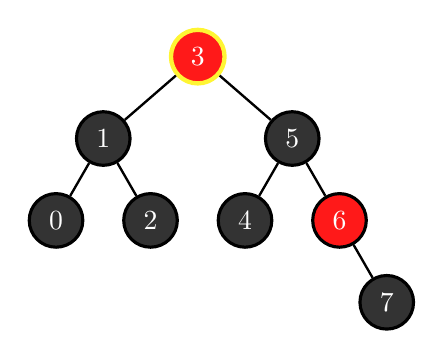
\begin{tikzpicture}[scale=0.8,
        level 1/.style={sibling distance=3cm},
        level 2/.style={sibling distance=1.5cm},
        ]
        \node[red, highlight] (p) {3}
          child{node[black] (c) {1}
            child{node[black] {0}}
            child{node[black] {2}}
          }
          child{node[black] {5}
            child{node[black] {4}}
            child{node[red] {6}
              child[missing]
              child{node[black] {7}}
            }
          };
      \end{tikzpicture}
    \end{minipage}
    \pause
    \begin{minipage}{0.2\textwidth}
      \begin{center}
        red root! $\mapsto$
      \end{center}
    \end{minipage}
    \begin{minipage}{0.39\textwidth}
      \centering
      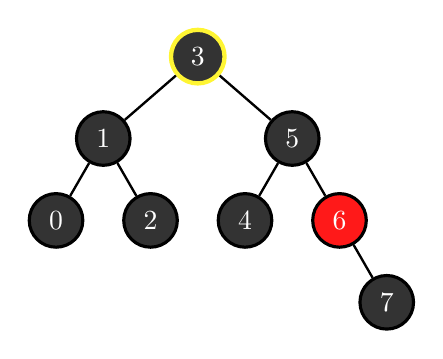
\begin{tikzpicture}[scale=0.8,
        level 1/.style={sibling distance=3cm},
        level 2/.style={sibling distance=1.5cm},
        ]
        \node[black, highlight] (p) {3}
          child{node[black] (c) {1}
            child{node[black] {0}}
            child{node[black] {2}}
          }
          child{node[black] {5}
            child{node[black] {4}}
            child{node[red] {6}
              child[missing]
              child{node[black] {7}}
            }
          };
      \end{tikzpicture}
    \end{minipage}
  \end{center}
\end{frame}

\begin{frame}[fragile]
  \frametitle{A Final Trace}

  \begin{center}
    \begin{minipage}{0.44\textwidth}
      \raggedright
      Now, we obtain a full RBT!
    \end{minipage}
    \begin{minipage}{0.4\textwidth}
      \goodbox{
        \node[black] (p) {3}
          child{node[black] (c) {1}
            child{node[black] {0}}
            child{node[black] {2}}
          }
          child{node[black] {5}
            child{node[black] {4}}
            child{node[red] {6}
              child[missing]
              child{node[black] {7}}
            }
          };
      }{
        scale=0.8,
        level 1/.style={sibling distance=3cm},
        level 2/.style={sibling distance=1.5cm},
      }
    \end{minipage}
  \end{center}
\end{frame}

% \begin{frame}[plain]
% 	\begin{center} Thank you! \end{center}

% 	\begin{center}
%     {\color{blue} \href{https://docs.google.com/forms/d/e/1FAIpQLSeuWVRsHKsKLdm0YIQBSbxIhdp4lozuzs90zZfY0QKmrJDPtA/viewform?usp=sf_link}{Post-lecture survey:}} \\
%     \vspace{5pt}
%     \includegraphics[scale=0.035]{qr_july13} \\
%     \vspace{5pt}
%     And the House Quiz winner is...
%   \end{center}
% \end{frame}

\thankyou

\end{document}
